%%%%%%%%%%%%%%%%%%%%%%%%%%%%%%%%%%%%%%
%%%%%%%%%%%%%%%%%%%%%%%%%%%%%%%%%%%%%%
% Do not edit the TeX file your work
% will be overwritten.  Edit the RnW
% file instead.
%%%%%%%%%%%%%%%%%%%%%%%%%%%%%%%%%%%%%%
%%%%%%%%%%%%%%%%%%%%%%%%%%%%%%%%%%%%%%





\newcommand{\ARMNumModels}{53}
\newcommand{\MCParamDim}{124}
\newcommand{\OccParamDim}{1,884}
\newcommand{\PotusParamDim}{15,098}
\newcommand{\TennisParamDim}{5,014}
\newcommand{\ARMMinParamDim}{2}
\newcommand{\ARMMedParamDim}{5}
\newcommand{\ARMMaxParamDim}{176}
\newcommand{\TennisNUTSMinutes}{57}
\newcommand{\PotusNUTSMinutes}{643}
\newcommand{\MCNUTSMinutes}{597}
\newcommand{\OccNUTSMinutes}{251}
\newcommand{\ARMMinNUTSSeconds}{15}
\newcommand{\ARMMedNUTSSeconds}{39}
\newcommand{\ARMMaxNUTSMinutes}{16}
\newcommand{\DADVINumDraws}{30}
\newcommand{\CoverageNumBins}{100}
\newcommand{\CoverageNumBinsPotus}{95}
\newcommand{\ArmModels}{wells\_dist100 (2), nes2000\_vote (2), separation (2), wells\_d100ars (3), earn\_height (3), electric\_one\_pred (3), radon\_complete\_pool (3), sesame\_one\_pred\_2b (3), logearn\_height (3), kidscore\_momhs (3), kidscore\_momiq (3), sesame\_one\_pred\_a (3), earnings1 (3), sesame\_one\_pred\_b (3), electric\_multi\_preds (4), earnings2 (4), kidiq\_multi\_preds (4), wells\_interaction\_c (4), wells\_interaction (4), wells\_dae (4), congress (4), logearn\_height\_male (4), logearn\_logheight (4), mesquite\_volume (5), logearn\_interaction (5), earnings\_interactions (5), ideo\_reparam (5), wells\_dae\_inter (5), wells\_dae\_c (5), kidscore\_momwork (5), kidiq\_interaction (5), wells\_daae\_c (6), wells\_dae\_inter\_c (7), mesquite\_vash (7), wells\_predicted\_log (7), mesquite\_log (8), mesquite\_vas (8), mesquite (8), sesame\_multi\_preds\_3b (9), sesame\_multi\_preds\_3a (9), pilots (17), election88 (53), radon\_intercept (88), radon\_no\_pool (89), radon\_group (90), electric (100), electric\_1b (101), electric\_1a (109), electric\_1c (114), hiv (170), hiv\_inter (171), radon\_vary\_si (174), radon\_inter\_vary (176)}
\newcommand{\TennisNumCGParams}{20}
\newcommand{\OccNumCGParams}{20}


%%%%%%%%%%%%%%%%%%%%%%
%%%%%%%%%%%%%%%%%%%%%%
%%%%%%%%%%%%%%%%%%%%%%
% Figures and tables



\newcommand{\TracesARM}{

\begin{knitrout}
\definecolor{shadecolor}{rgb}{0.969, 0.969, 0.969}\color{fgcolor}\begin{figure}[!h]

{\centering 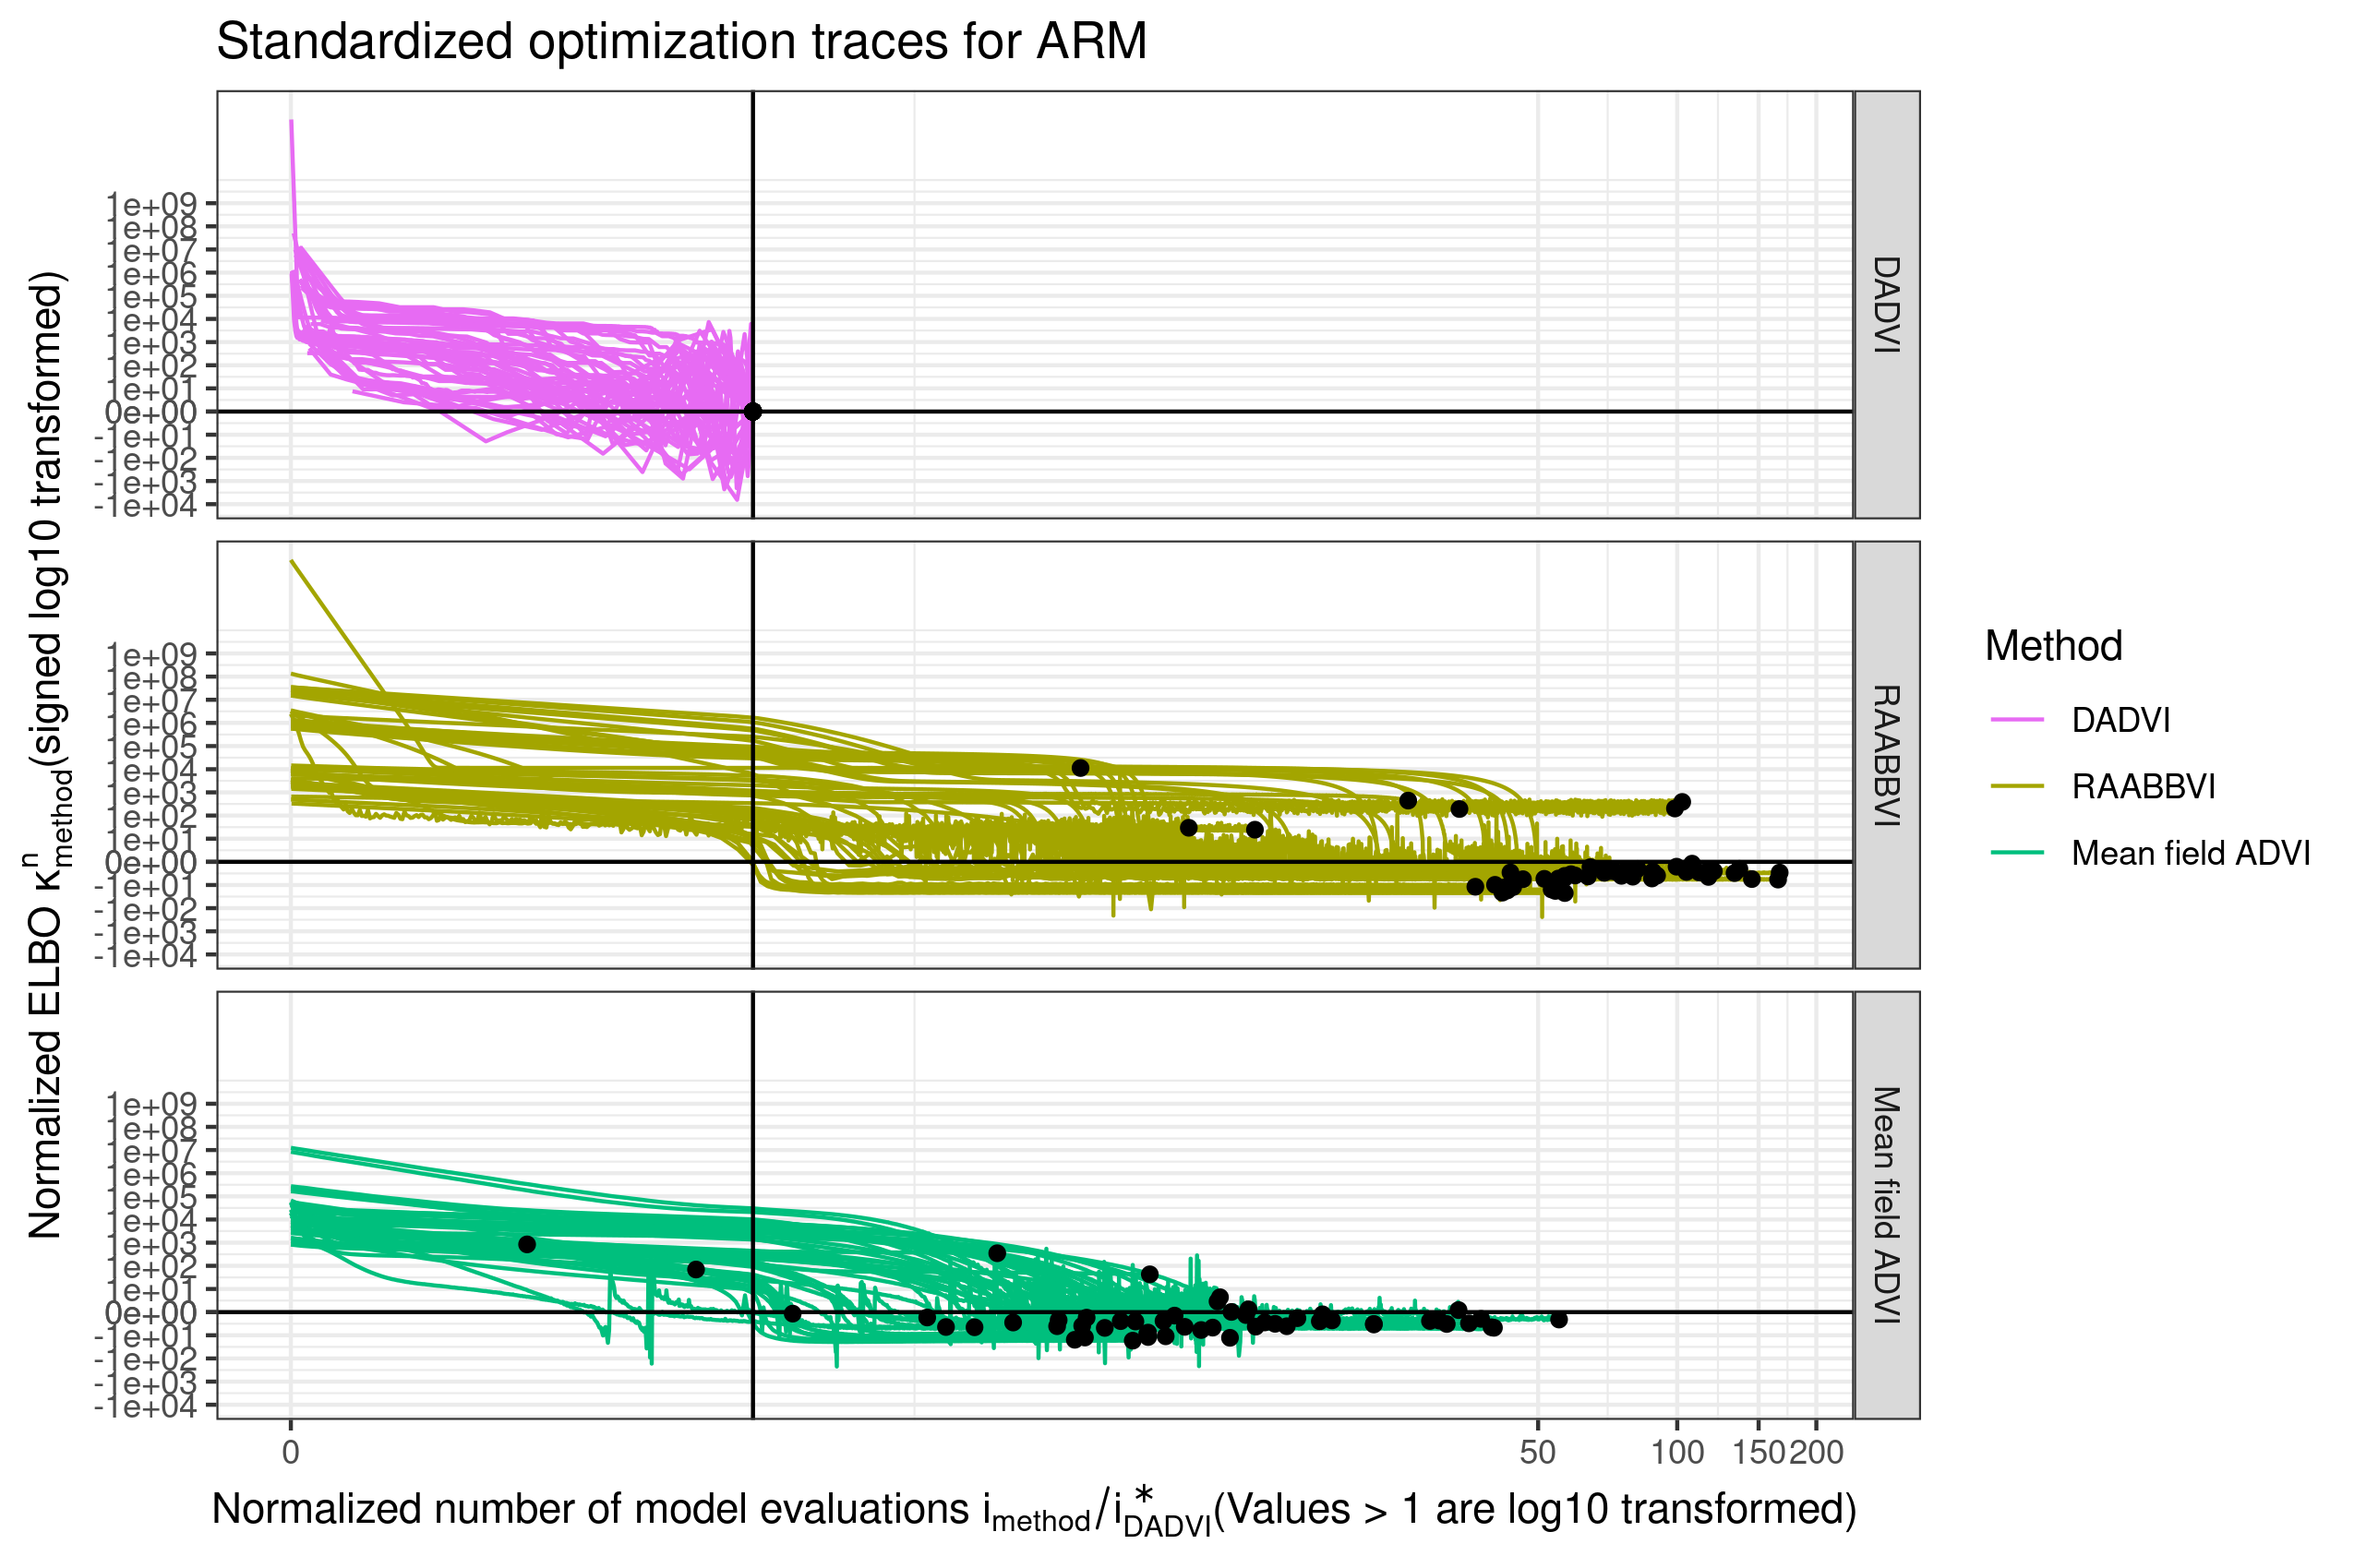
\includegraphics[width=0.98\linewidth,height=0.653\linewidth]{figure/traces_arm_graph-1} 

}

\caption[Optimization traces for the ARM models]{Optimization traces for the ARM models.  Black dots show the termination point of each method. Dots above the horizontal black line mean that DADVI found a better ELBO. Dots to the right of the black line mean that DADVI terminated sooner in terms of model evaluations.}\label{fig:traces_arm_graph}
\end{figure}

\end{knitrout}
}


\newcommand{\TracesNonARM}{

\begin{knitrout}
\definecolor{shadecolor}{rgb}{0.969, 0.969, 0.969}\color{fgcolor}\begin{figure}[!h]

{\centering 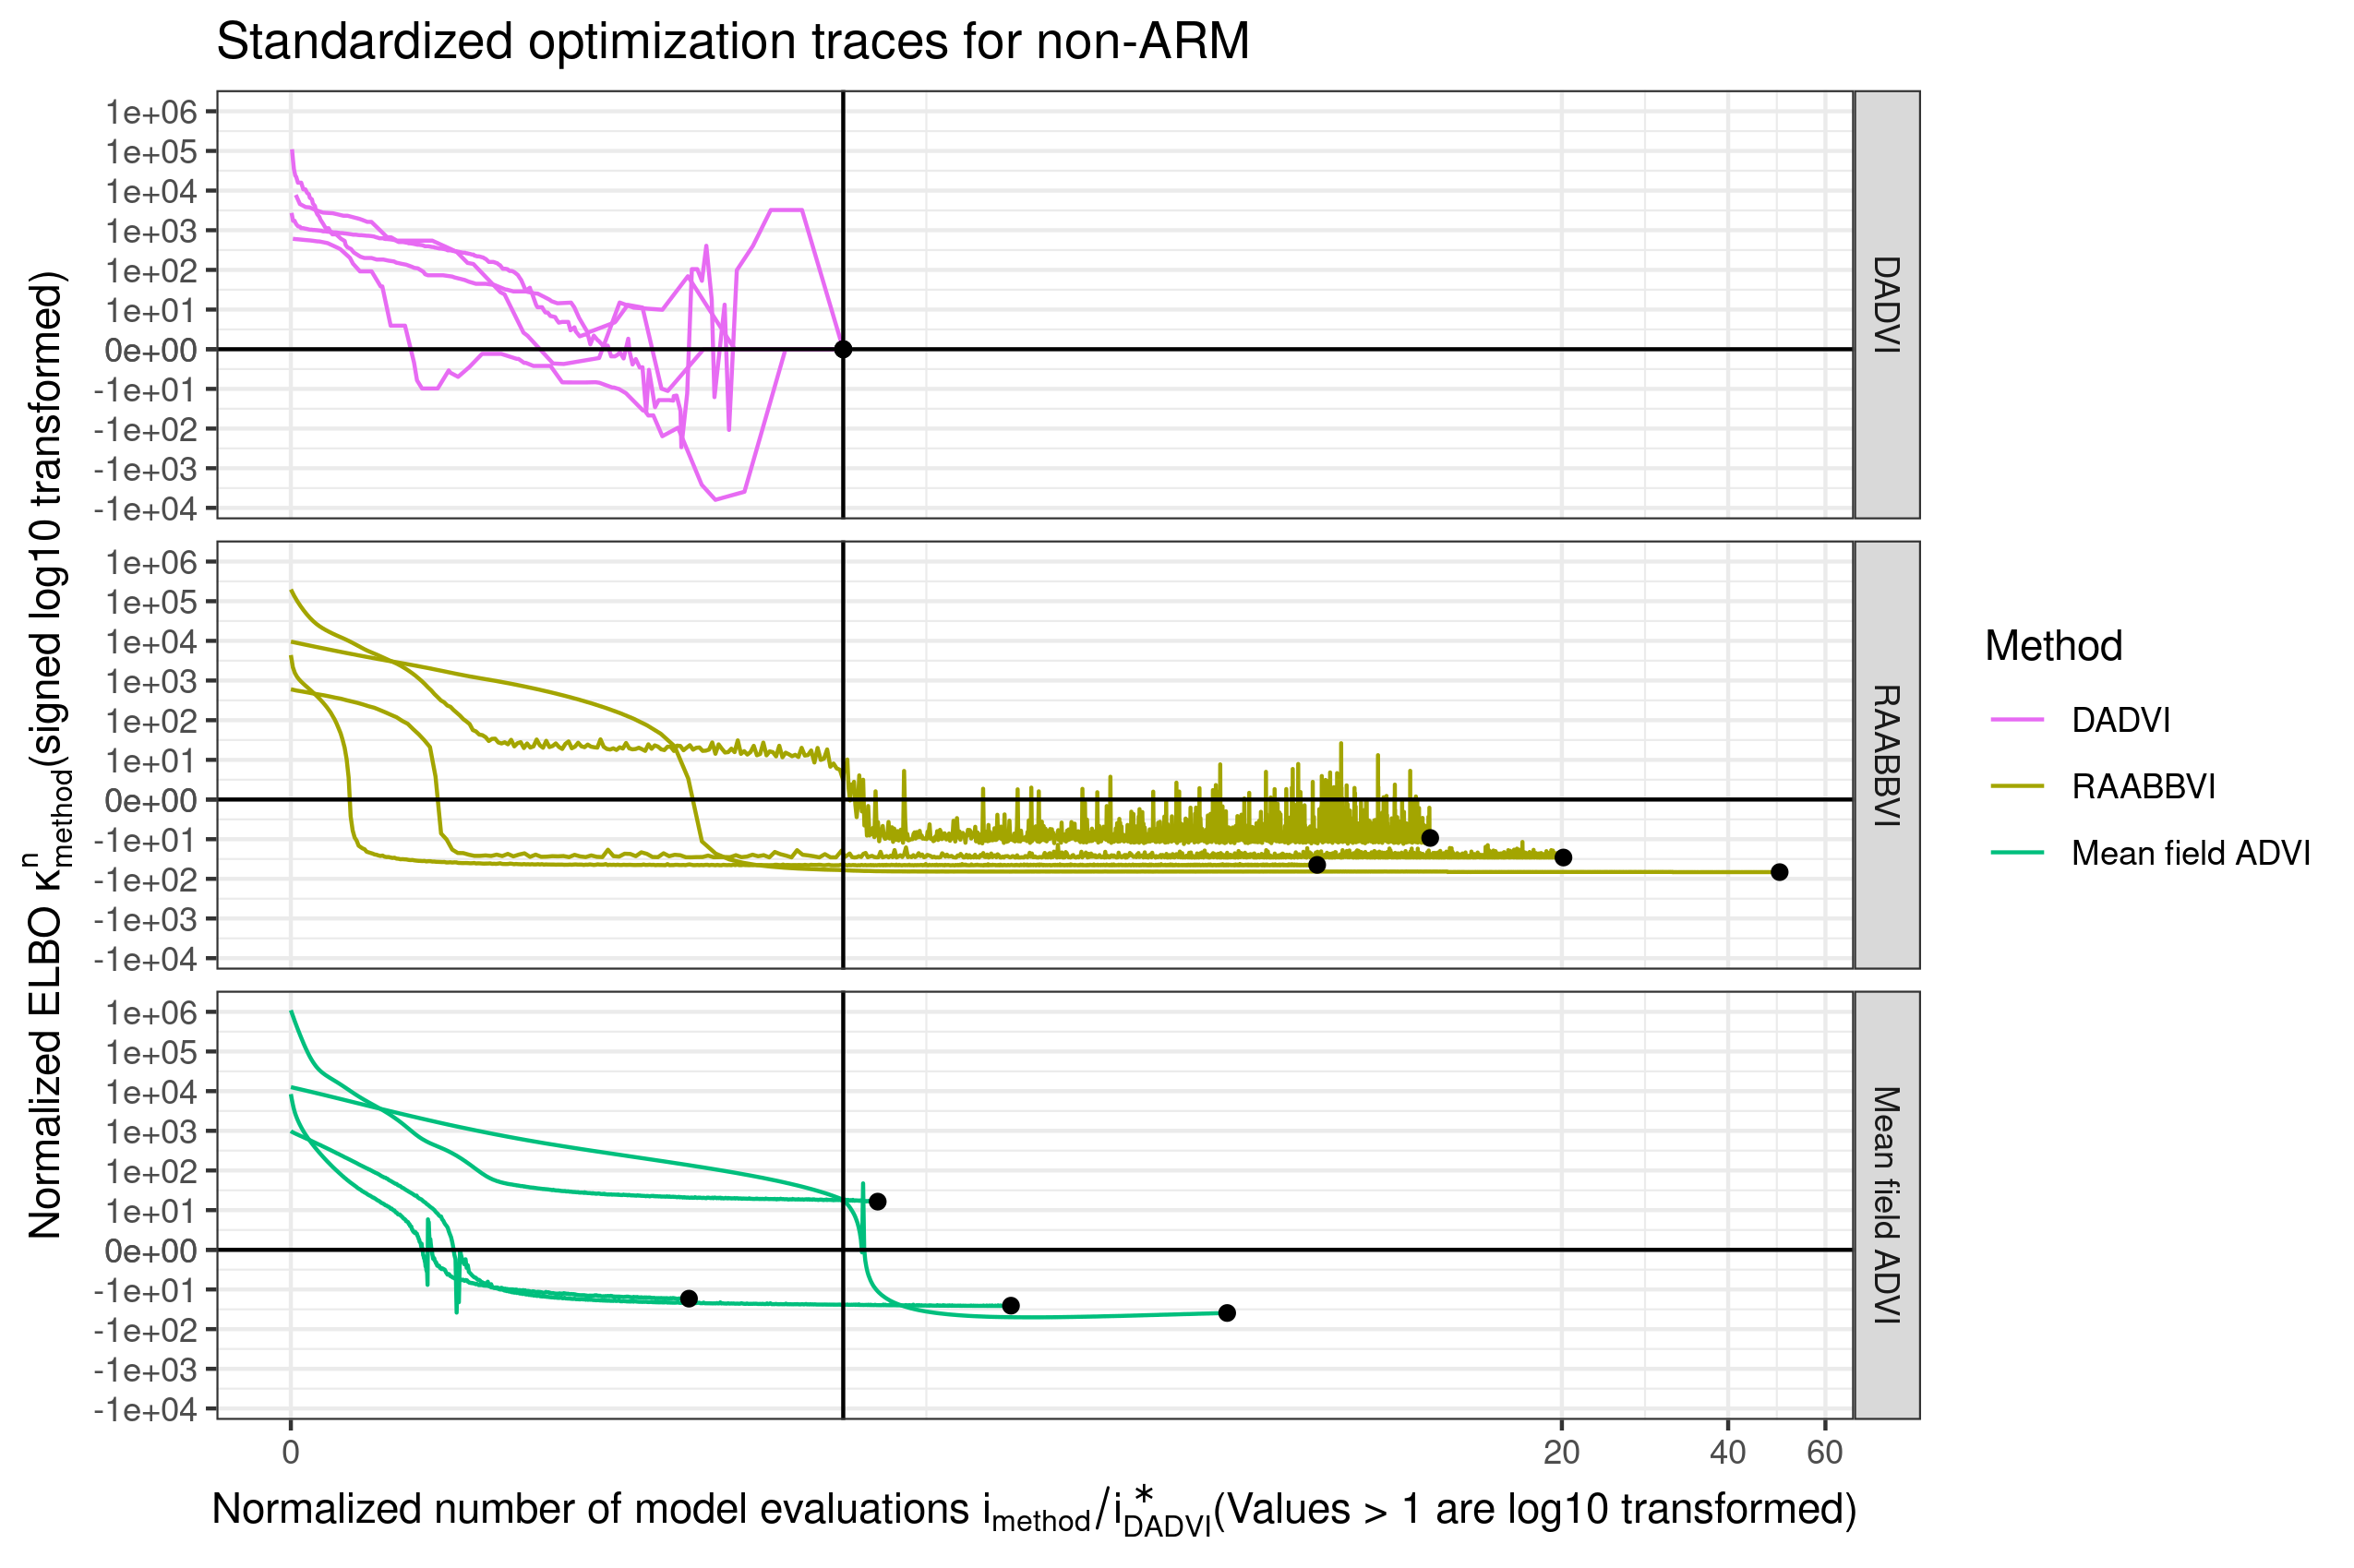
\includegraphics[width=0.98\linewidth,height=0.653\linewidth]{figure/traces_nonarm_graph-1} 

}

\caption[Traces for non-ARM models]{Traces for non-ARM models.  Black dots show the termination point of each method. Dots above the horizontal black line mean that DADVI found a better ELBO. Dots to the right of the black line mean that DADVI terminated sooner in terms of model evaluations.}\label{fig:traces_nonarm_graph}
\end{figure}

\end{knitrout}
}




\newcommand{\RuntimeARM}{

\begin{knitrout}
\definecolor{shadecolor}{rgb}{0.969, 0.969, 0.969}\color{fgcolor}\begin{figure}[!h]

{\centering 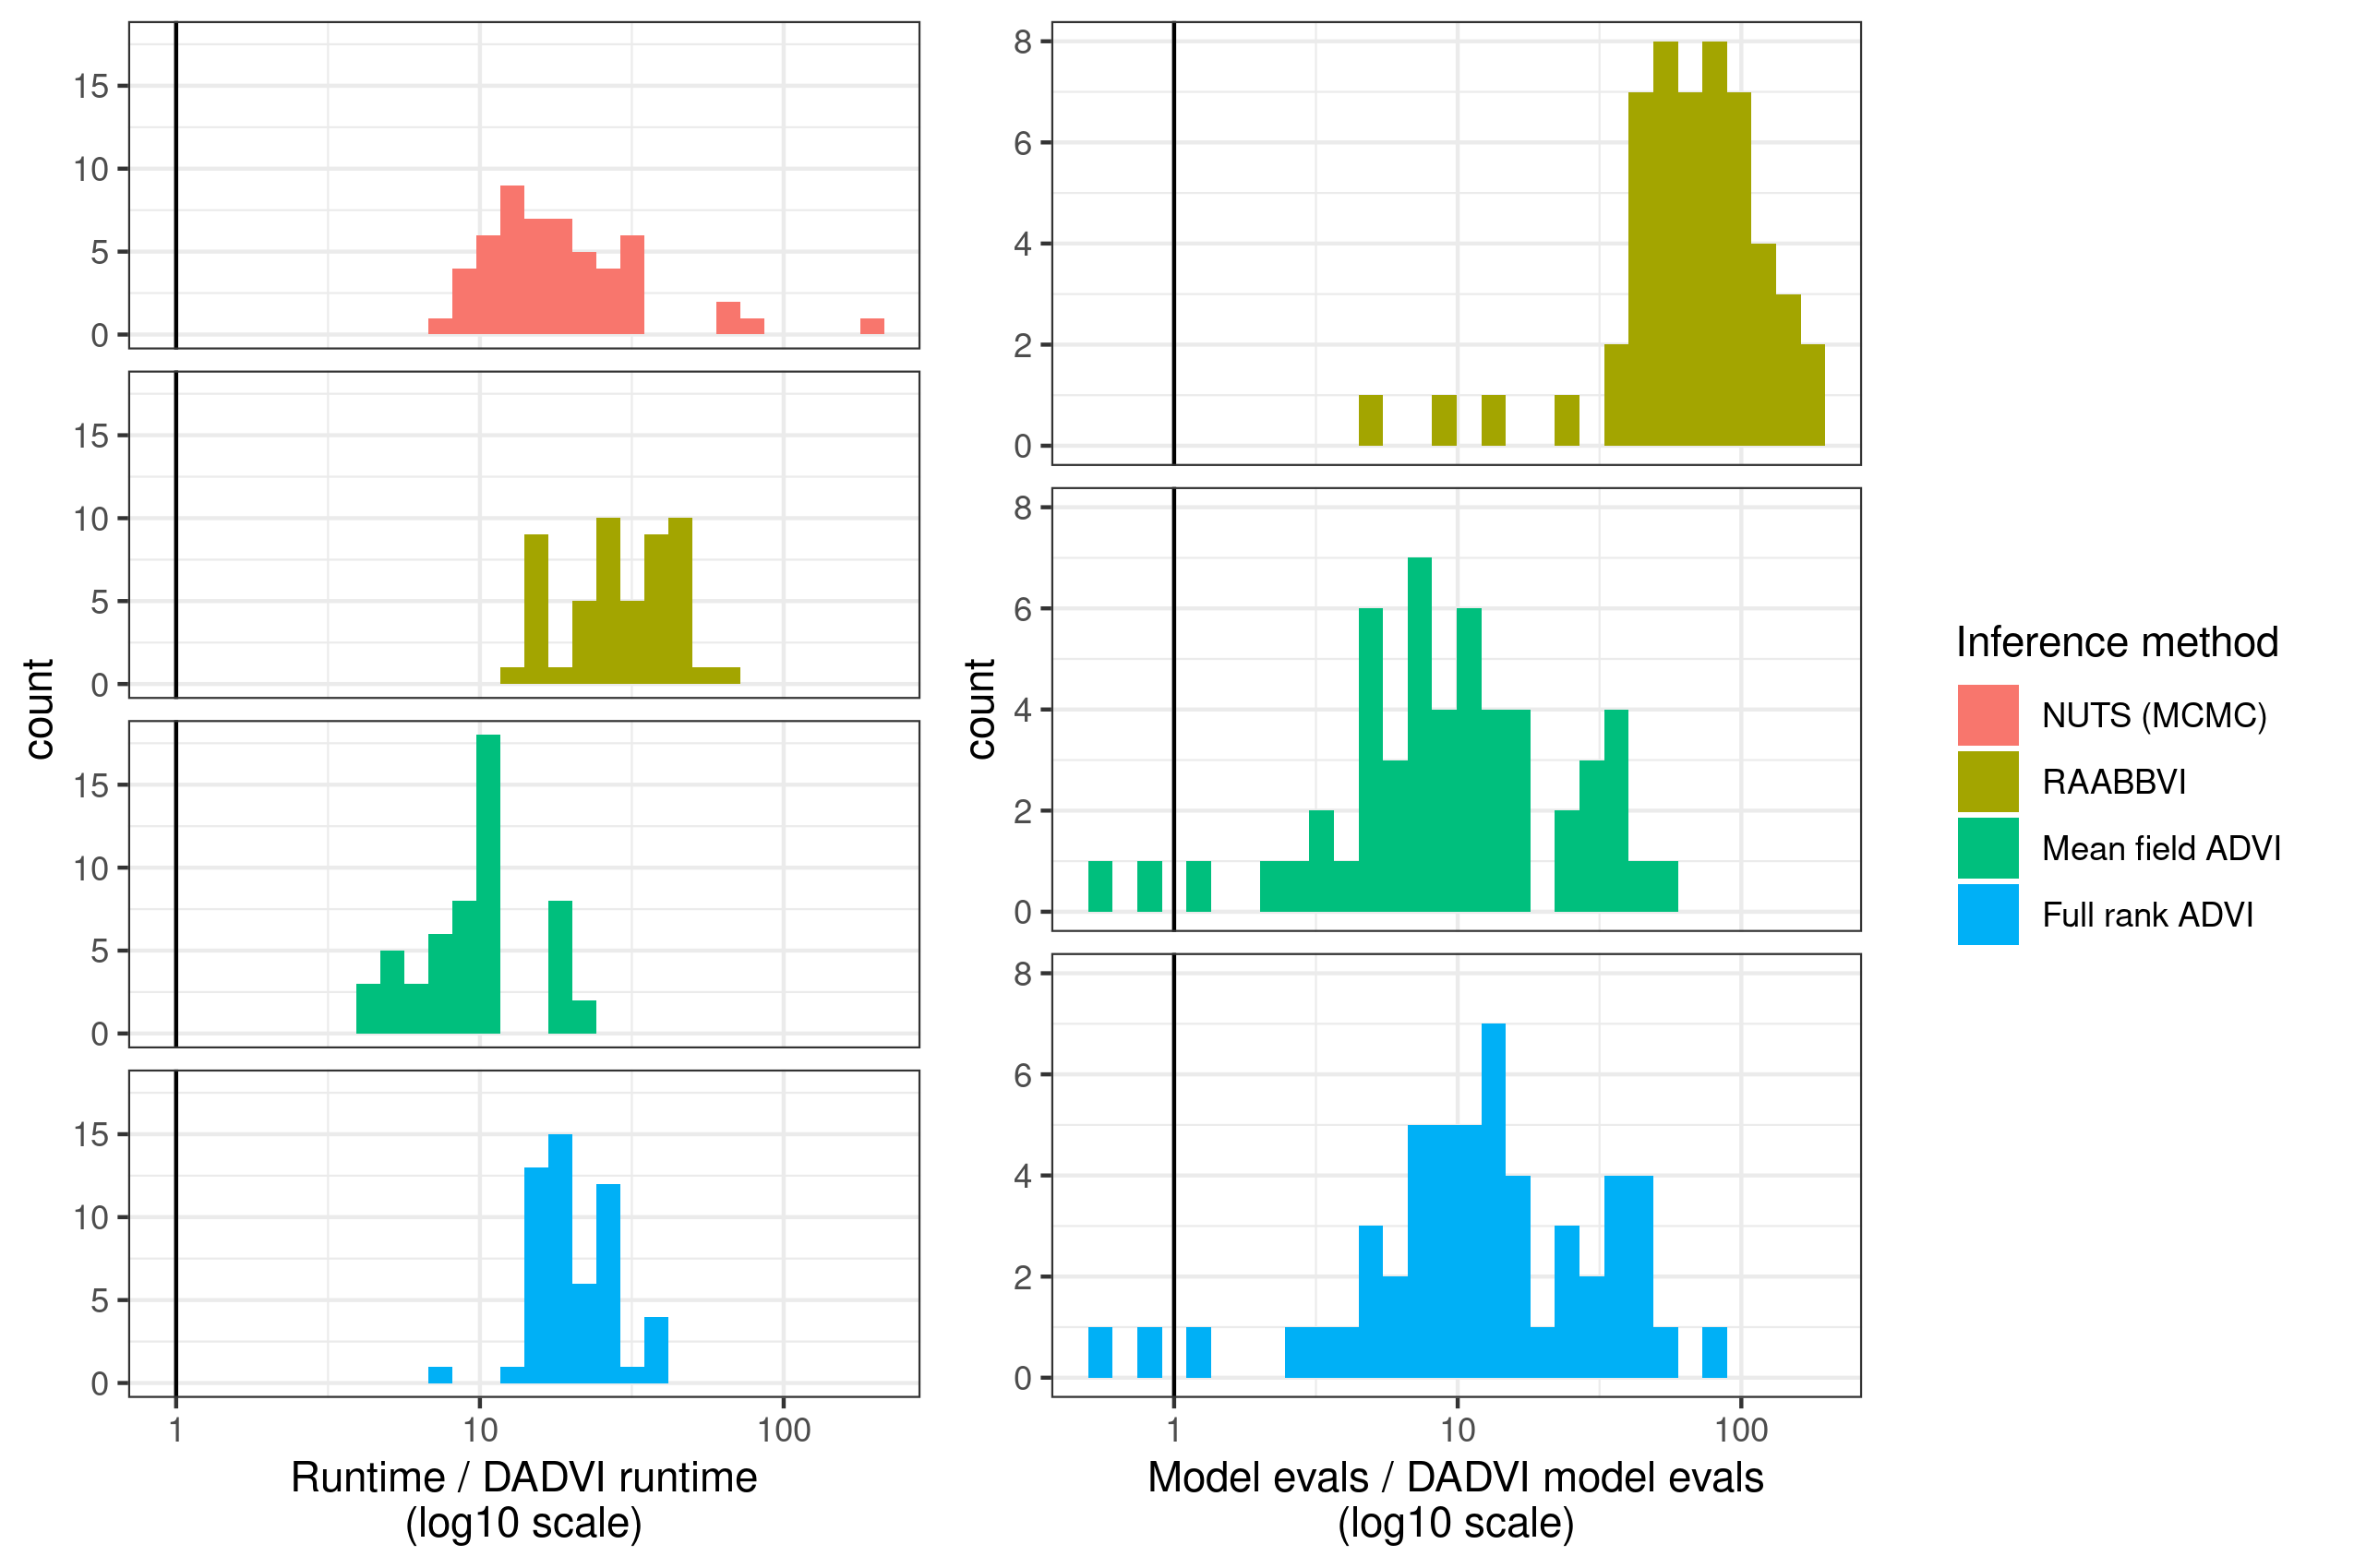
\includegraphics[width=0.98\linewidth,height=0.653\linewidth]{figure/runtimes_arm_graph-1} 

}

\caption[Runtimes and model evaluation counts for the ARM models]{Runtimes and model evaluation counts for the ARM models. Results are reported divided by the corresponding value for DADVI.}\label{fig:runtimes_arm_graph}
\end{figure}

\end{knitrout}
}



\newcommand{\RuntimeNonARM}{

\begin{knitrout}
\definecolor{shadecolor}{rgb}{0.969, 0.969, 0.969}\color{fgcolor}\begin{figure}[!h]

{\centering 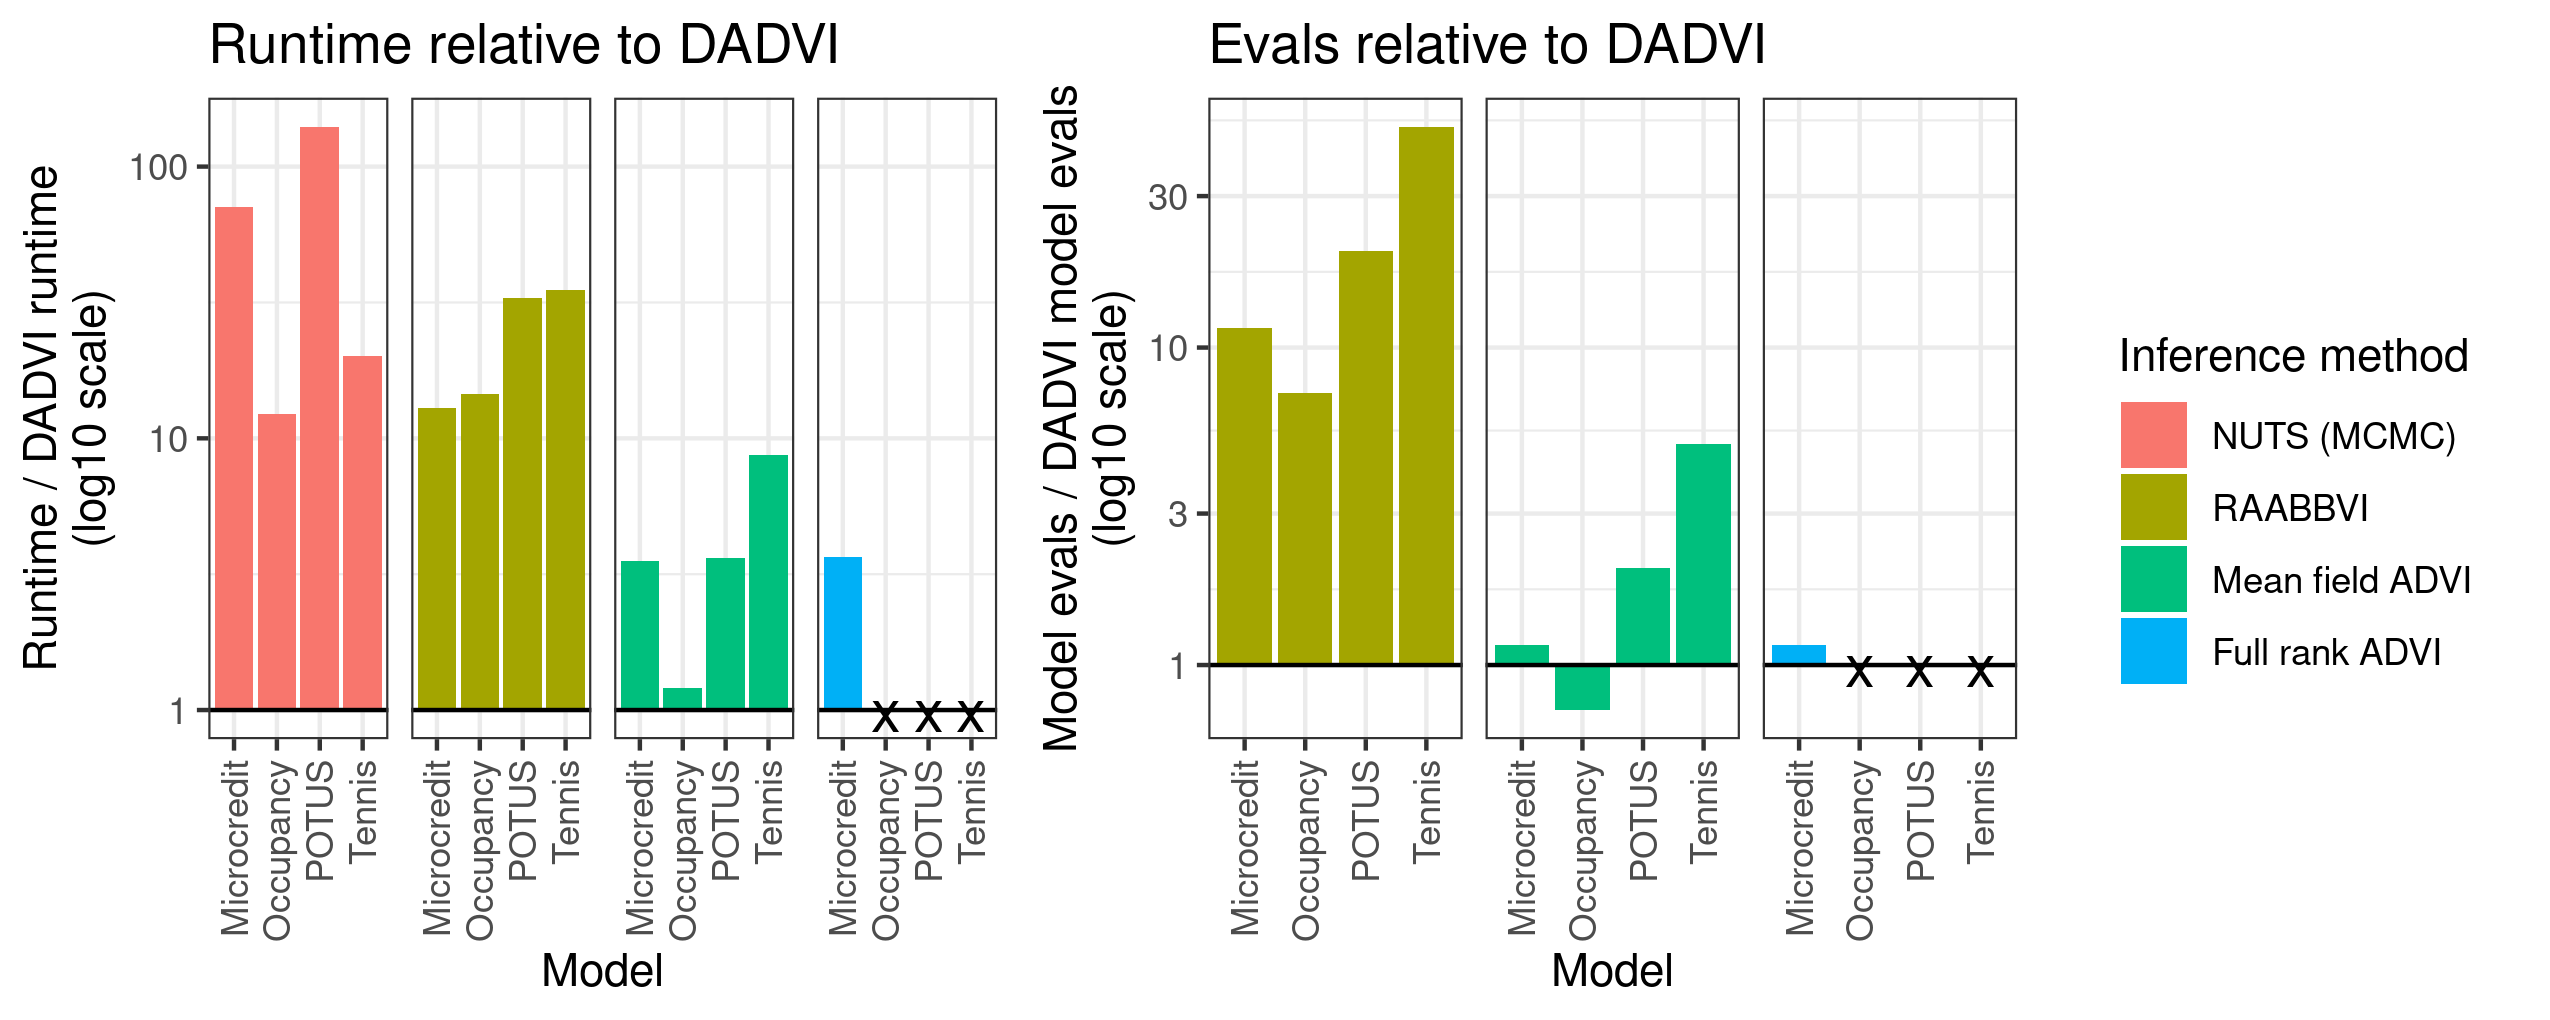
\includegraphics[width=0.98\linewidth,height=0.392\linewidth]{figure/runtimes_nonarm_graph-1} 

}

\caption[Runtimes and model evaluation counts for the non-ARM models]{Runtimes and model evaluation counts for the non-ARM models. Results are reported divided by the corresponding value for DADVI. Missing model / method combinations are marked with an X.}\label{fig:runtimes_nonarm_graph}
\end{figure}

\end{knitrout}
}






% \newcommand{\PosteriorAccuracyARM}{
% <<posterior_arm_graph_cap>>=
% figcap <- paste0(
%     "Posterior accuracy measures for the ARM models. ",
%     GetPostComparisonText(), " ",
%     "Level curves of a 2D density estimator are shown to help visualize ",
%     "overplotting.")
% SetImageSize()
% @
% <<posterior_arm_graph, cache=knitr_cache, fig.show='hold', fig.cap=figcap>>=
% source("figures_knitr/posterior_comparison_arm.R",
%        echo=knitr_debug, print.eval=TRUE)
% @
% }


% \newcommand{\PosteriorAccuracyNonARM}{
% <<posterior_nonarm_graph_cap>>=
% figcap <- paste0(
%     "Posterior accuracy measures for the non-ARM models. ",
%     GetPostComparisonText())
% SetImageSize()
% @
% <<posterior_nonarm_graph, cache=knitr_cache, fig.show='hold', fig.cap=figcap>>=
% source("figures_knitr/posterior_comparison_nonarm.R",
%        echo=knitr_debug, print.eval=TRUE)
% @
% }




\newcommand{\PosteriorMeanAccuracy}{

\begin{knitrout}
\definecolor{shadecolor}{rgb}{0.969, 0.969, 0.969}\color{fgcolor}\begin{figure}[!h]

{\centering 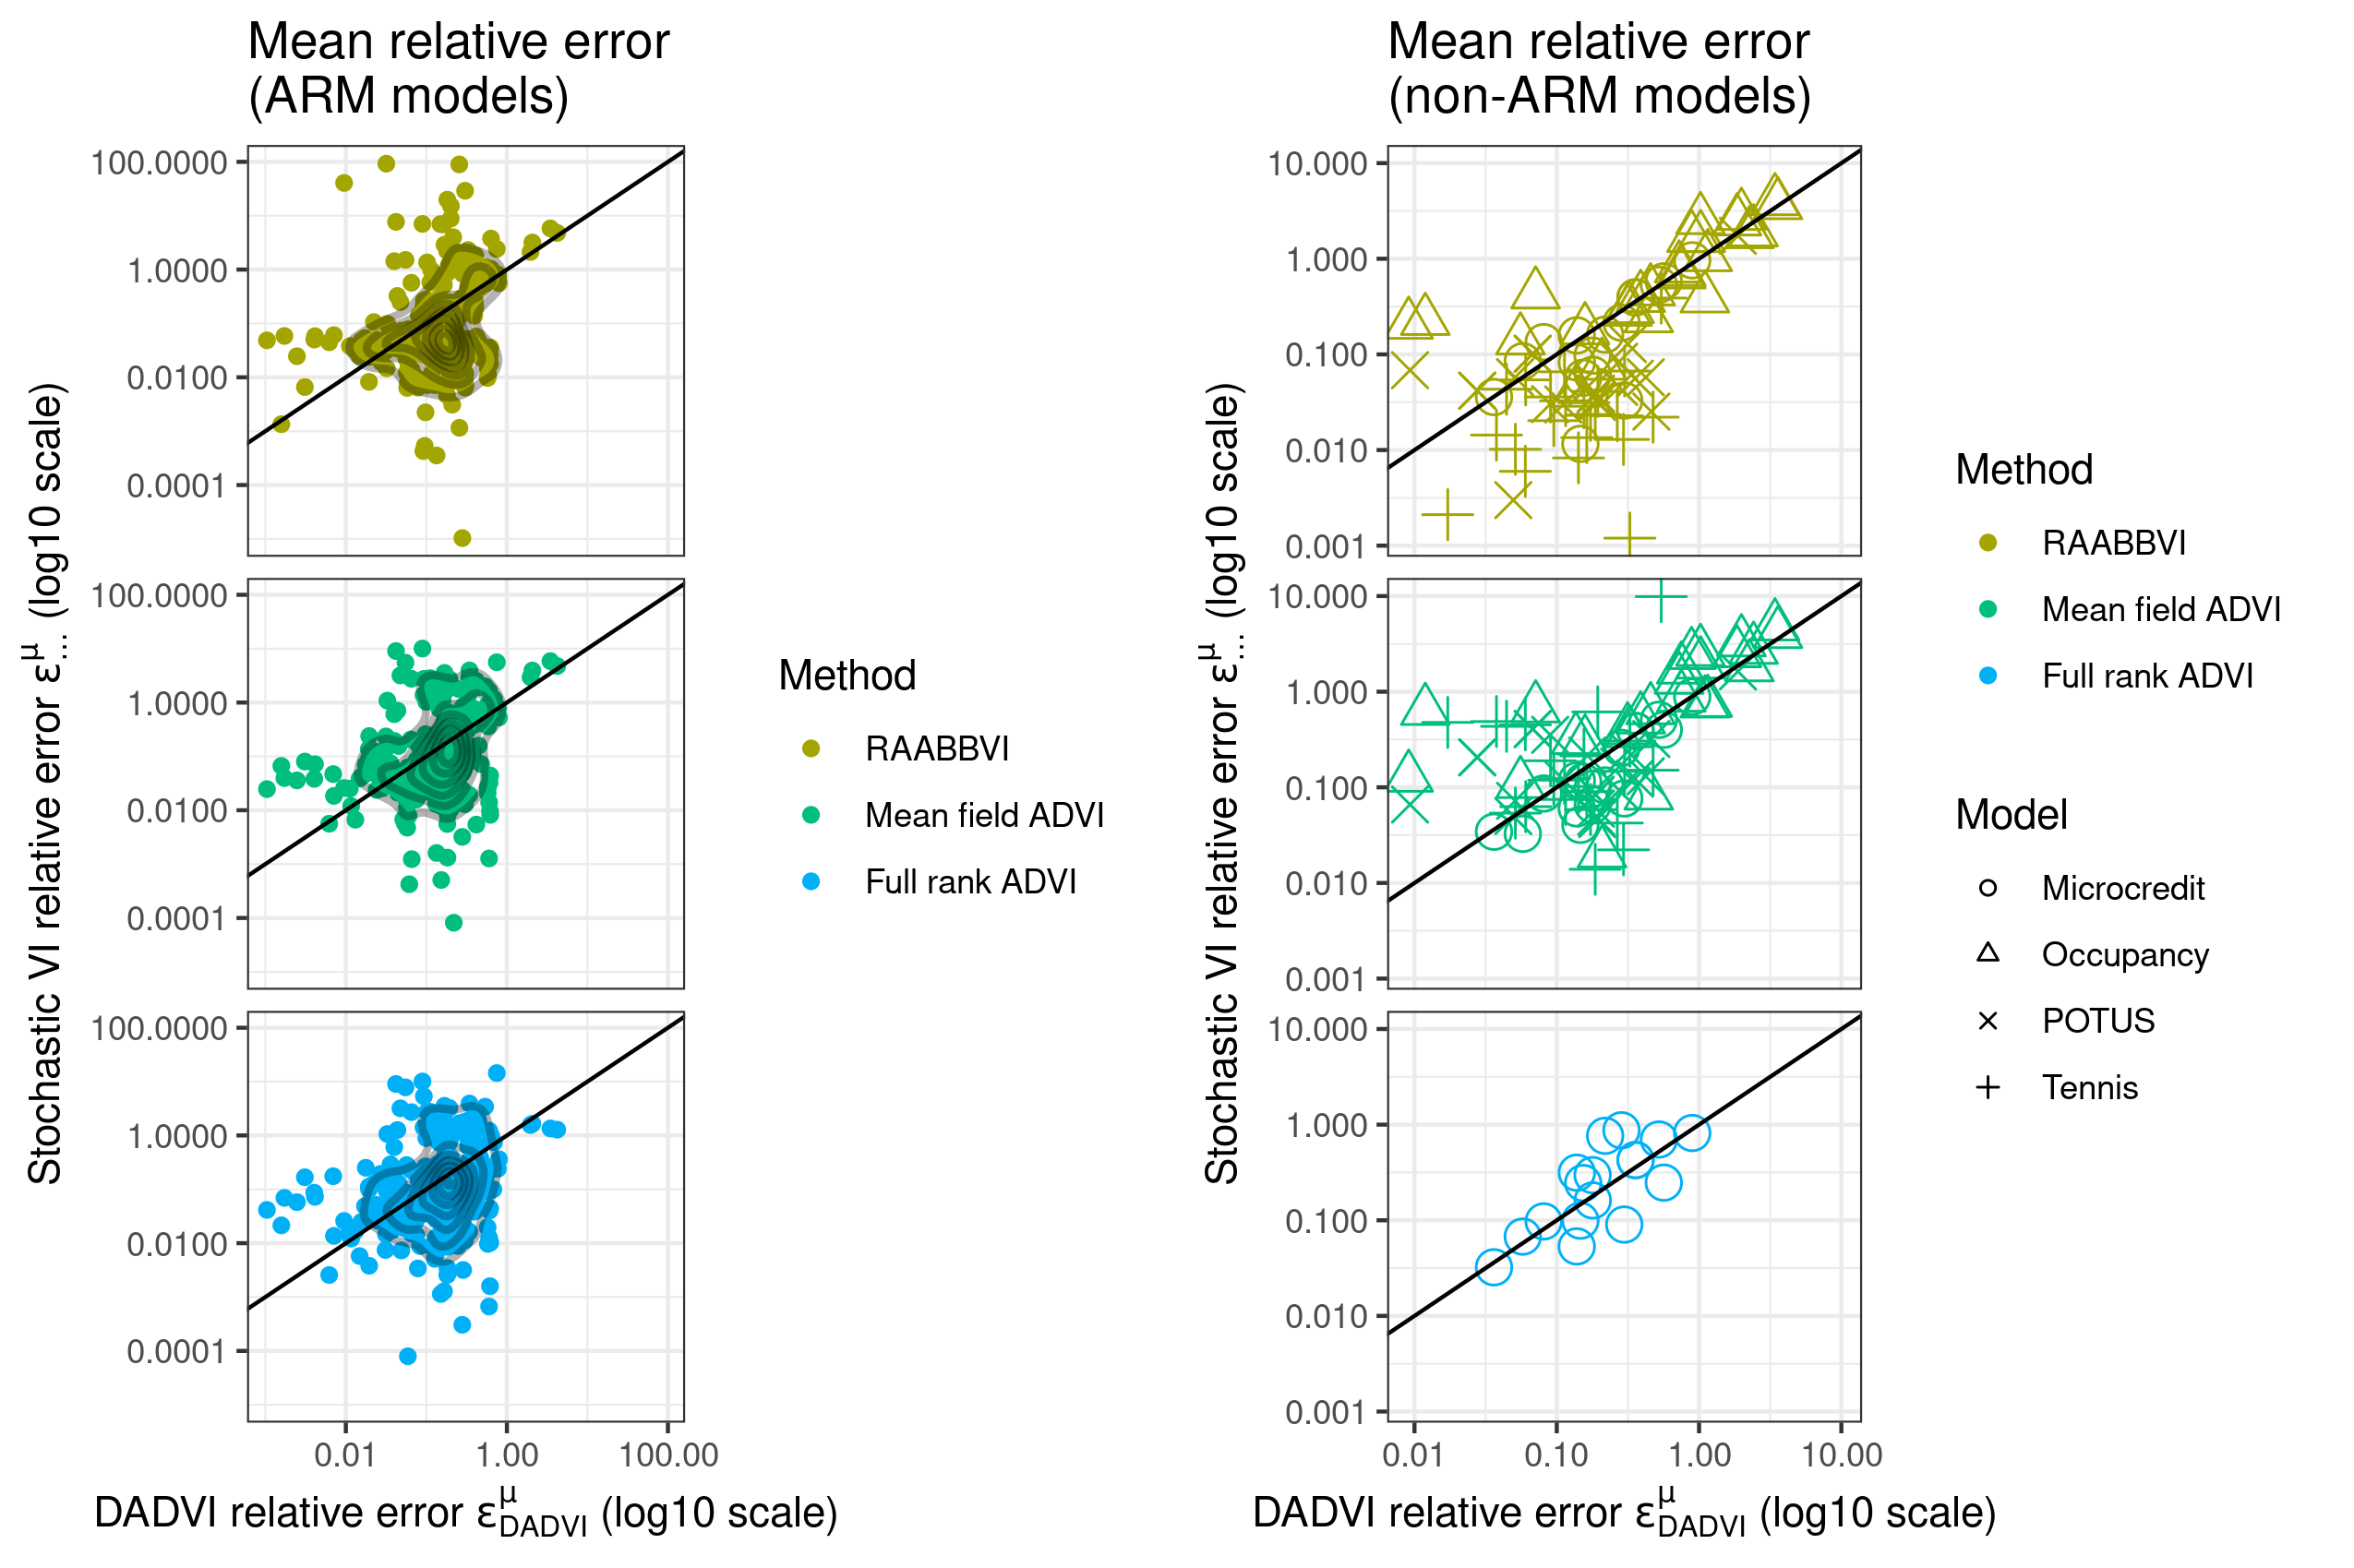
\includegraphics[width=0.98\linewidth,height=0.653\linewidth]{figure/posterior_mean_graph-1} 

}

\caption[Posterior mean accuracy (relative to MCMC posterior standard deviation)]{Posterior mean accuracy (relative to MCMC posterior standard deviation). Each point is a single named parameter in a single model. Points above the diagonal line indicate better DADVI or LRVB performance. }\label{fig:posterior_mean_graph}
\end{figure}

\end{knitrout}
}




\newcommand{\PosteriorSdAccuracy}{

\begin{knitrout}
\definecolor{shadecolor}{rgb}{0.969, 0.969, 0.969}\color{fgcolor}\begin{figure}[!h]

{\centering 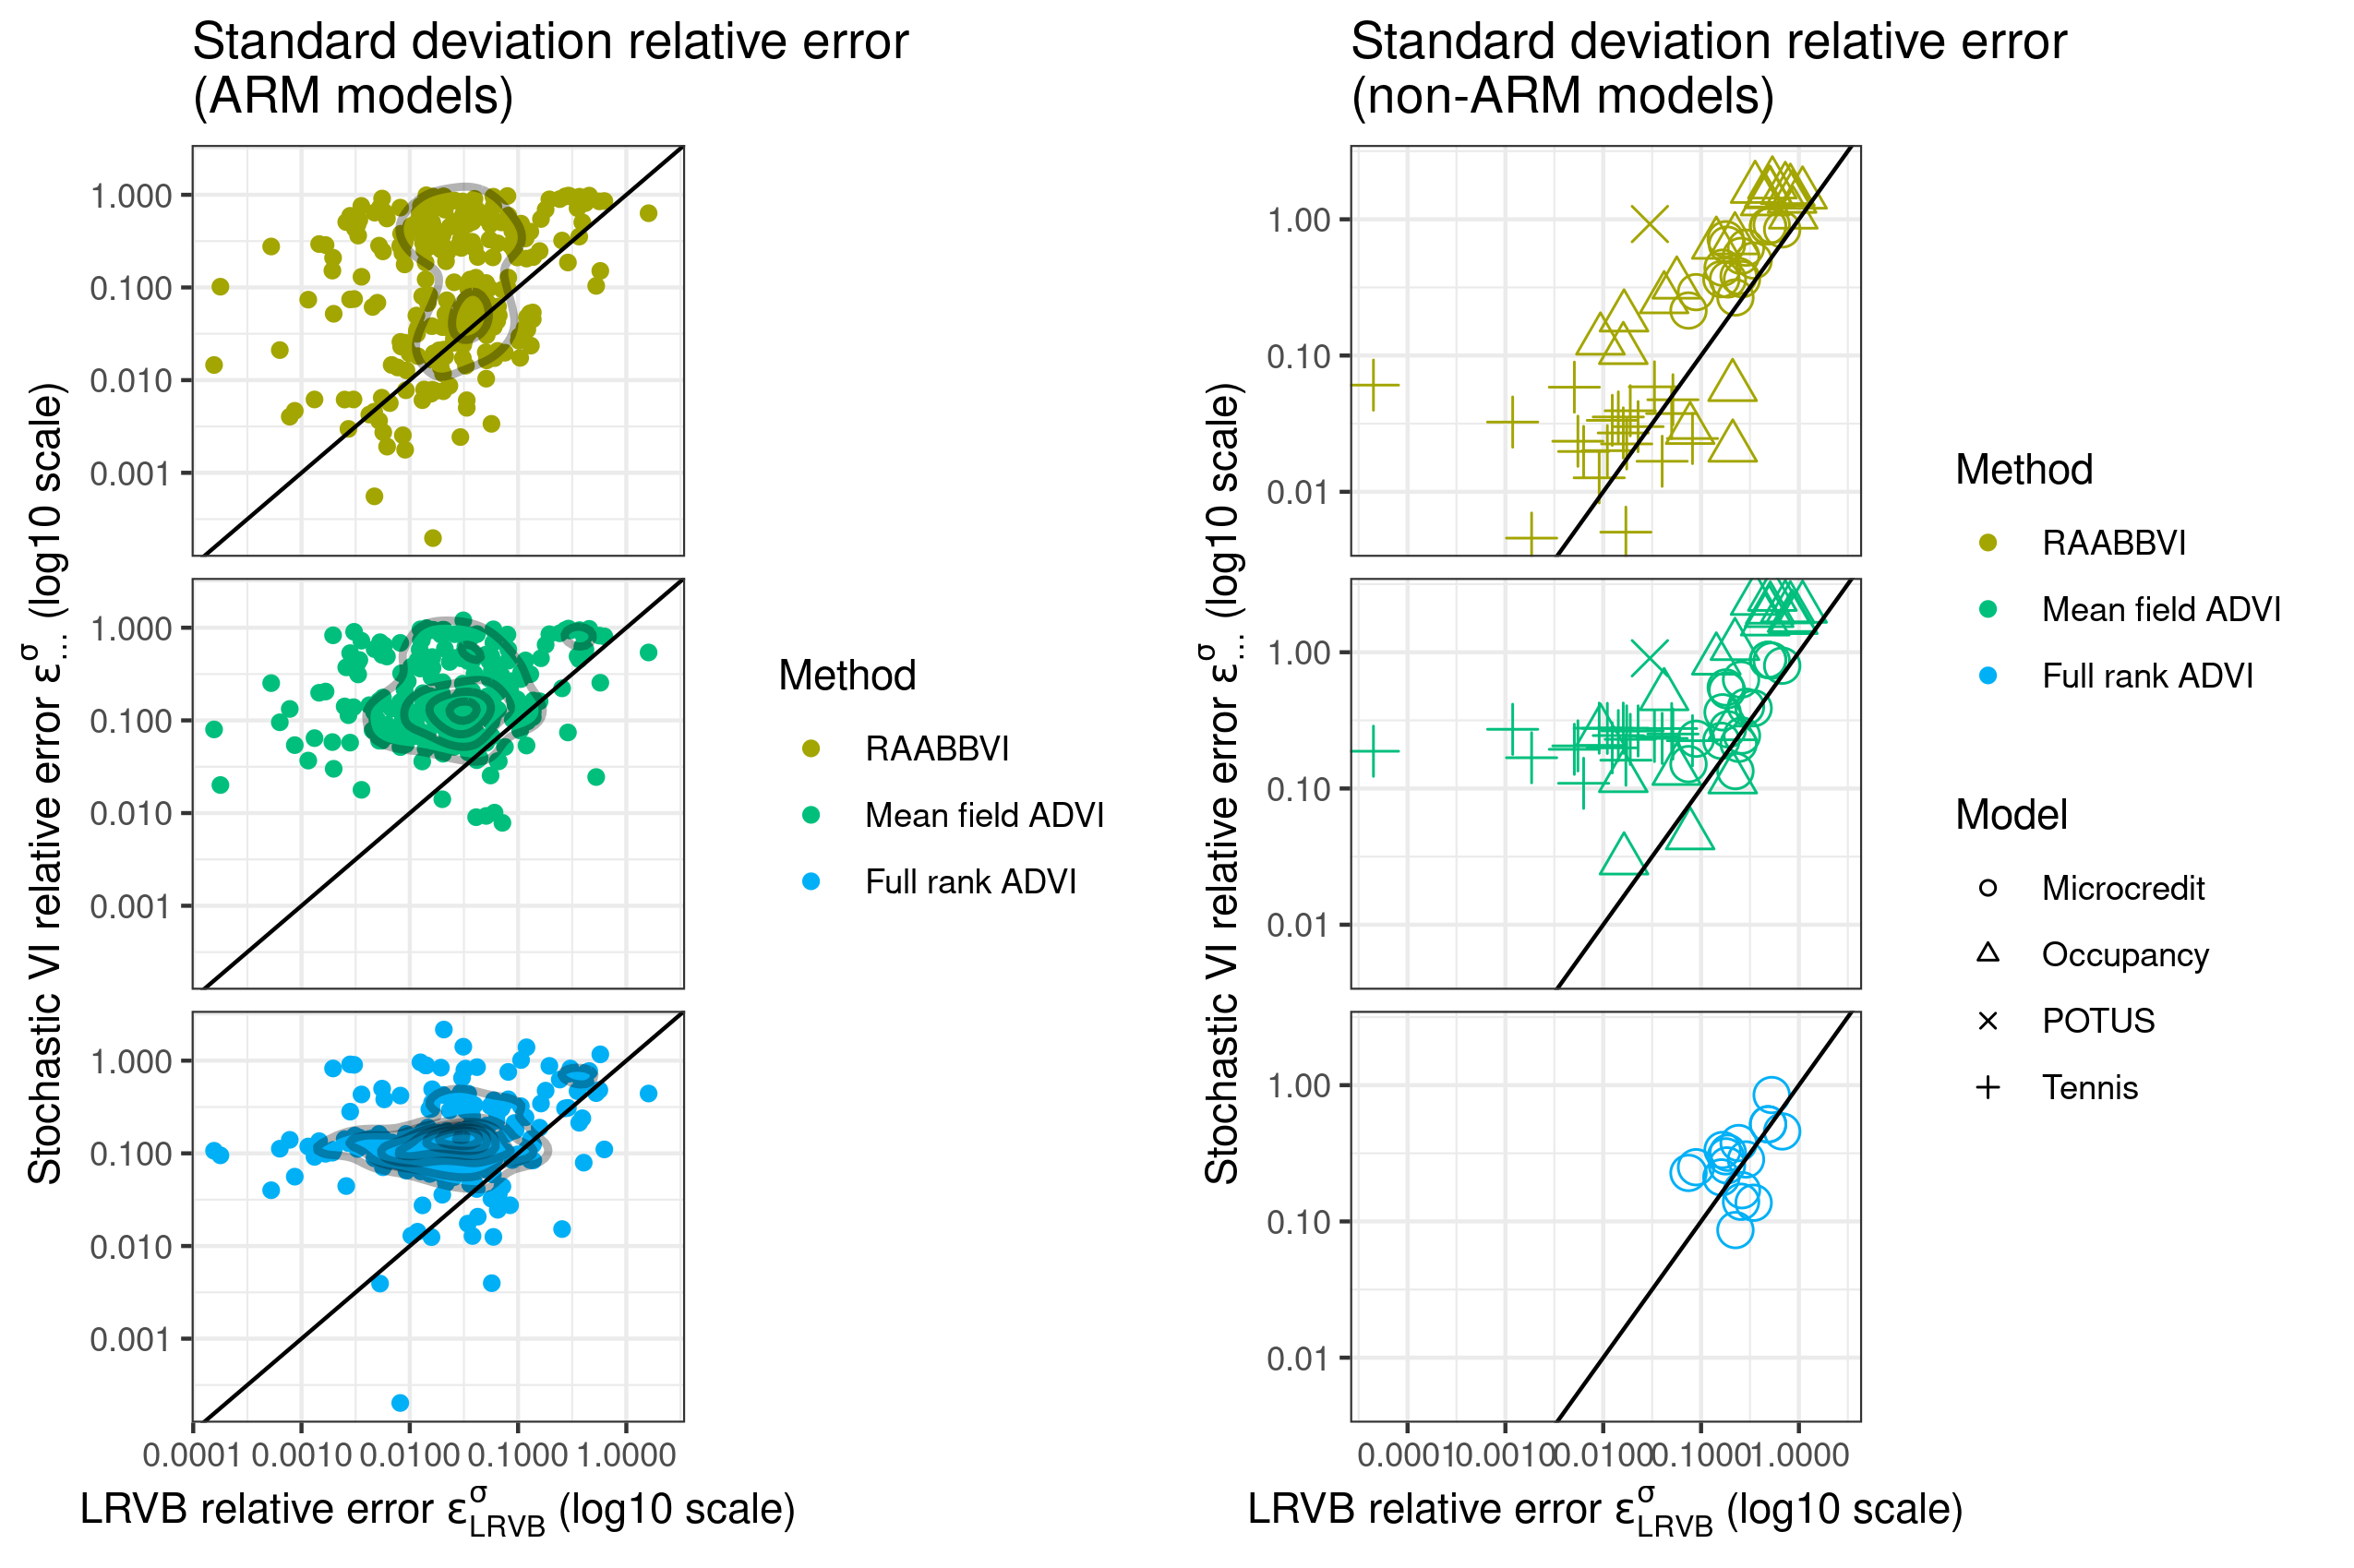
\includegraphics[width=0.98\linewidth,height=0.653\linewidth]{figure/posterior_sd_graph-1} 

}

\caption[Posterior sd relative accuracy]{Posterior sd relative accuracy. Each point is a single named parameter in a single model. Points above the diagonal line indicate better DADVI or LRVB performance. }\label{fig:posterior_sd_graph}
\end{figure}

\end{knitrout}
}

%%%%%%%%%%%%%%%%%%%%%%%%%%%%%%%%%%%%%%%%%%%%%%%%%%%%%%%%%%%%%%%%%%%%%%%%%%




\newcommand{\CoverageHistogram}{

\begin{knitrout}
\definecolor{shadecolor}{rgb}{0.969, 0.969, 0.969}\color{fgcolor}\begin{figure}[!h]

{\centering 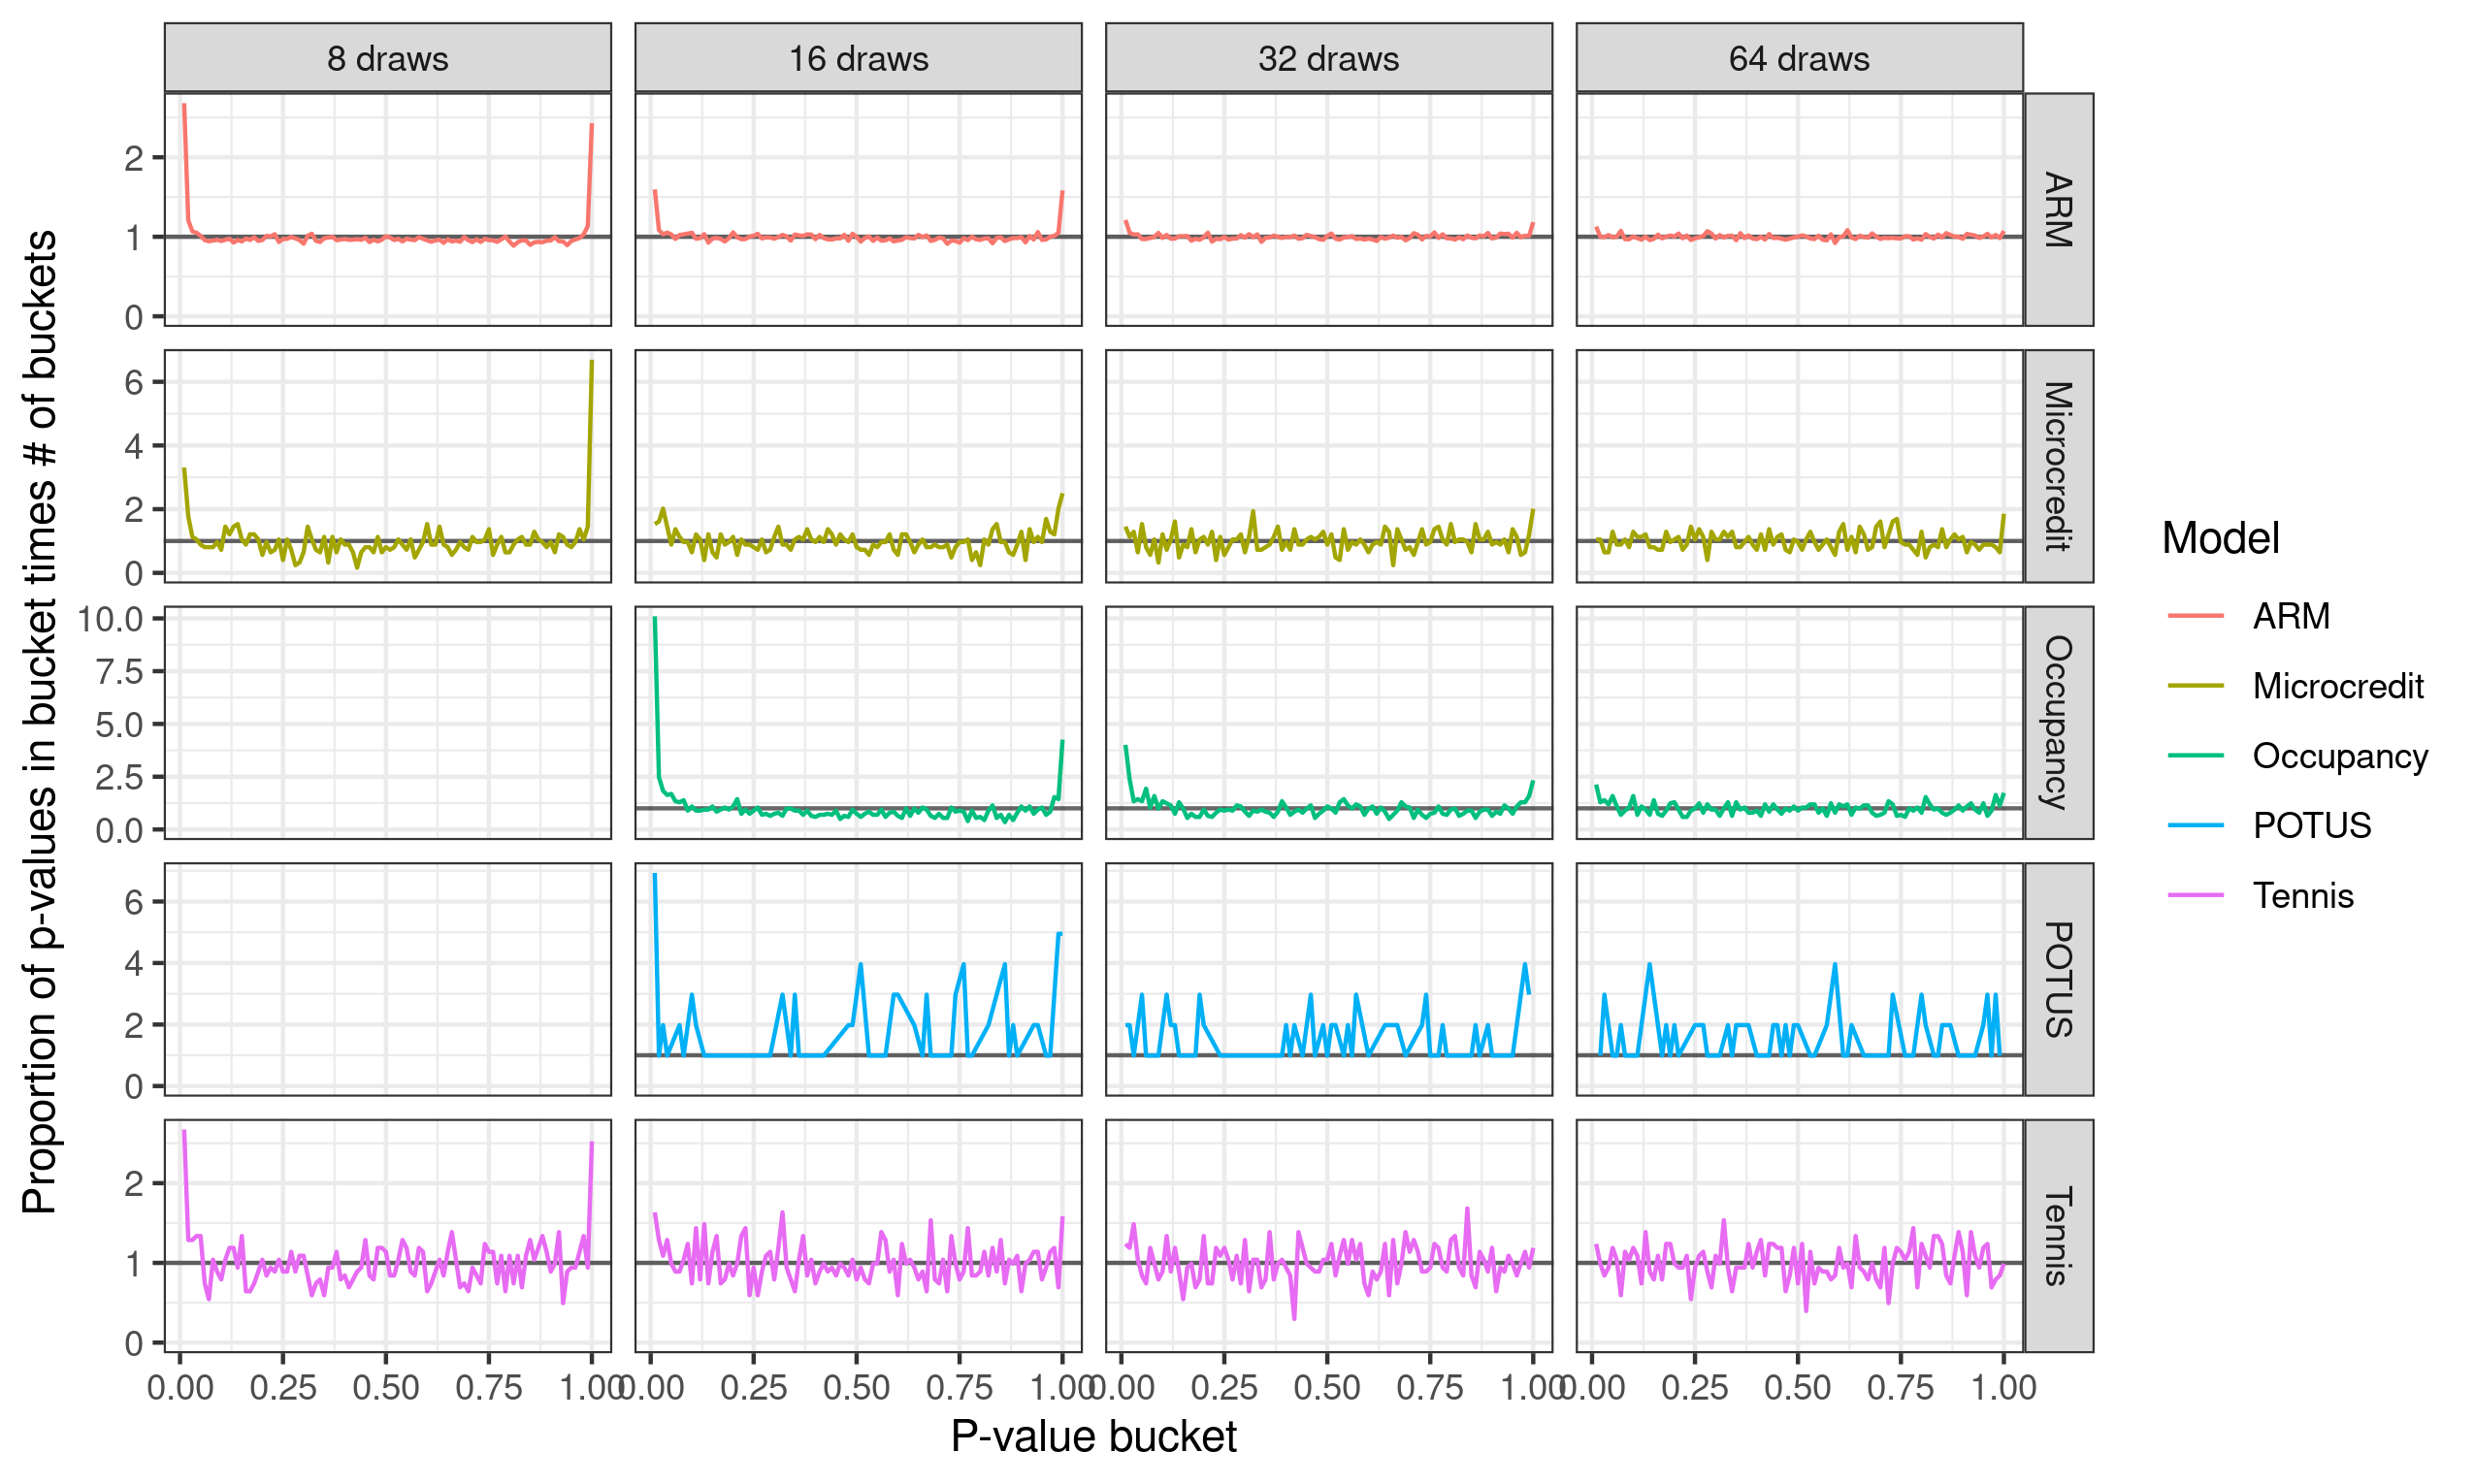
\includegraphics[width=0.98\linewidth,height=0.588\linewidth]{figure/coverage-1} 

}

\caption[Density estimates of $\Phi(\freqerr)$ for difference models]{Density estimates of $\Phi(\freqerr)$ for difference models. All the ARM models are grouped together for ease of visualization.  Each panel shows a binned estimate of the density of $\Phi(\freqerr)$ for a particular model and number of draws $\znum$. Values close to one (a uniform density) indicate good frequentist performance.  CG failed for the Occupancy and POTUS models with only 8 draws, possibly indicating poor optimization performance with so few samples.}\label{fig:coverage}
\end{figure}

\end{knitrout}
}
